\documentclass[1p]{elsarticle_modified}
%\bibliographystyle{elsarticle-num}

%\usepackage[colorlinks]{hyperref}
%\usepackage{abbrmath_seonhwa} %\Abb, \Ascr, \Acal ,\Abf, \Afrak
\usepackage{amsfonts}
\usepackage{amssymb}
\usepackage{amsmath}
\usepackage{amsthm}
\usepackage{scalefnt}
\usepackage{amsbsy}
\usepackage{kotex}
\usepackage{caption}
\usepackage{subfig}
\usepackage{color}
\usepackage{graphicx}
\usepackage{xcolor} %% white, black, red, green, blue, cyan, magenta, yellow
\usepackage{float}
\usepackage{setspace}
\usepackage{hyperref}

\usepackage{tikz}
\usetikzlibrary{arrows}

\usepackage{multirow}
\usepackage{array} % fixed length table
\usepackage{hhline}

%%%%%%%%%%%%%%%%%%%%%
\makeatletter
\renewcommand*\env@matrix[1][\arraystretch]{%
	\edef\arraystretch{#1}%
	\hskip -\arraycolsep
	\let\@ifnextchar\new@ifnextchar
	\array{*\c@MaxMatrixCols c}}
\makeatother %https://tex.stackexchange.com/questions/14071/how-can-i-increase-the-line-spacing-in-a-matrix
%%%%%%%%%%%%%%%

\usepackage[normalem]{ulem}

\newcommand{\msout}[1]{\ifmmode\text{\sout{\ensuremath{#1}}}\else\sout{#1}\fi}
%SOURCE: \msout is \stkout macro in https://tex.stackexchange.com/questions/20609/strikeout-in-math-mode

\newcommand{\cancel}[1]{
	\ifmmode
	{\color{red}\msout{#1}}
	\else
	{\color{red}\sout{#1}}
	\fi
}

\newcommand{\add}[1]{
	{\color{blue}\uwave{#1}}
}

\newcommand{\replace}[2]{
	\ifmmode
	{\color{red}\msout{#1}}{\color{blue}\uwave{#2}}
	\else
	{\color{red}\sout{#1}}{\color{blue}\uwave{#2}}
	\fi
}

\newcommand{\Sol}{\mathcal{S}} %segment
\newcommand{\D}{D} %diagram
\newcommand{\A}{\mathcal{A}} %arc


%%%%%%%%%%%%%%%%%%%%%%%%%%%%%5 test

\def\sl{\operatorname{\textup{SL}}(2,\Cbb)}
\def\psl{\operatorname{\textup{PSL}}(2,\Cbb)}
\def\quan{\mkern 1mu \triangleright \mkern 1mu}

\theoremstyle{definition}
\newtheorem{thm}{Theorem}[section]
\newtheorem{prop}[thm]{Proposition}
\newtheorem{lem}[thm]{Lemma}
\newtheorem{ques}[thm]{Question}
\newtheorem{cor}[thm]{Corollary}
\newtheorem{defn}[thm]{Definition}
\newtheorem{exam}[thm]{Example}
\newtheorem{rmk}[thm]{Remark}
\newtheorem{alg}[thm]{Algorithm}

\newcommand{\I}{\sqrt{-1}}
\begin{document}

%\begin{frontmatter}
%
%\title{Boundary parabolic representations of knots up to 8 crossings}
%
%%% Group authors per affiliation:
%\author{Yunhi Cho} 
%\address{Department of Mathematics, University of Seoul, Seoul, Korea}
%\ead{yhcho@uos.ac.kr}
%
%
%\author{Seonhwa Kim} %\fnref{s_kim}}
%\address{Center for Geometry and Physics, Institute for Basic Science, Pohang, 37673, Korea}
%\ead{ryeona17@ibs.re.kr}
%
%\author{Hyuk Kim}
%\address{Department of Mathematical Sciences, Seoul National University, Seoul 08826, Korea}
%\ead{hyukkim@snu.ac.kr}
%
%\author{Seokbeom Yoon}
%\address{Department of Mathematical Sciences, Seoul National University, Seoul, 08826,  Korea}
%\ead{sbyoon15@snu.ac.kr}
%
%\begin{abstract}
%We find all boundary parabolic representation of knots up to 8 crossings.
%
%\end{abstract}
%\begin{keyword}
%    \MSC[2010] 57M25 
%\end{keyword}
%
%\end{frontmatter}

%\linenumbers
%\tableofcontents
%
\newcommand\colored[1]{\textcolor{white}{\rule[-0.35ex]{0.8em}{1.4ex}}\kern-0.8em\color{red} #1}%
%\newcommand\colored[1]{\textcolor{white}{ #1}\kern-2.17ex	\textcolor{white}{ #1}\kern-1.81ex	\textcolor{white}{ #1}\kern-2.15ex\color{red}#1	}

{\Large $\underline{12a_{1191}~(K12a_{1191})}$}

\setlength{\tabcolsep}{10pt}
\renewcommand{\arraystretch}{1.6}
\vspace{1cm}\begin{tabular}{m{100pt}>{\centering\arraybackslash}m{274pt}}
\multirow{5}{120pt}{
	\centering
	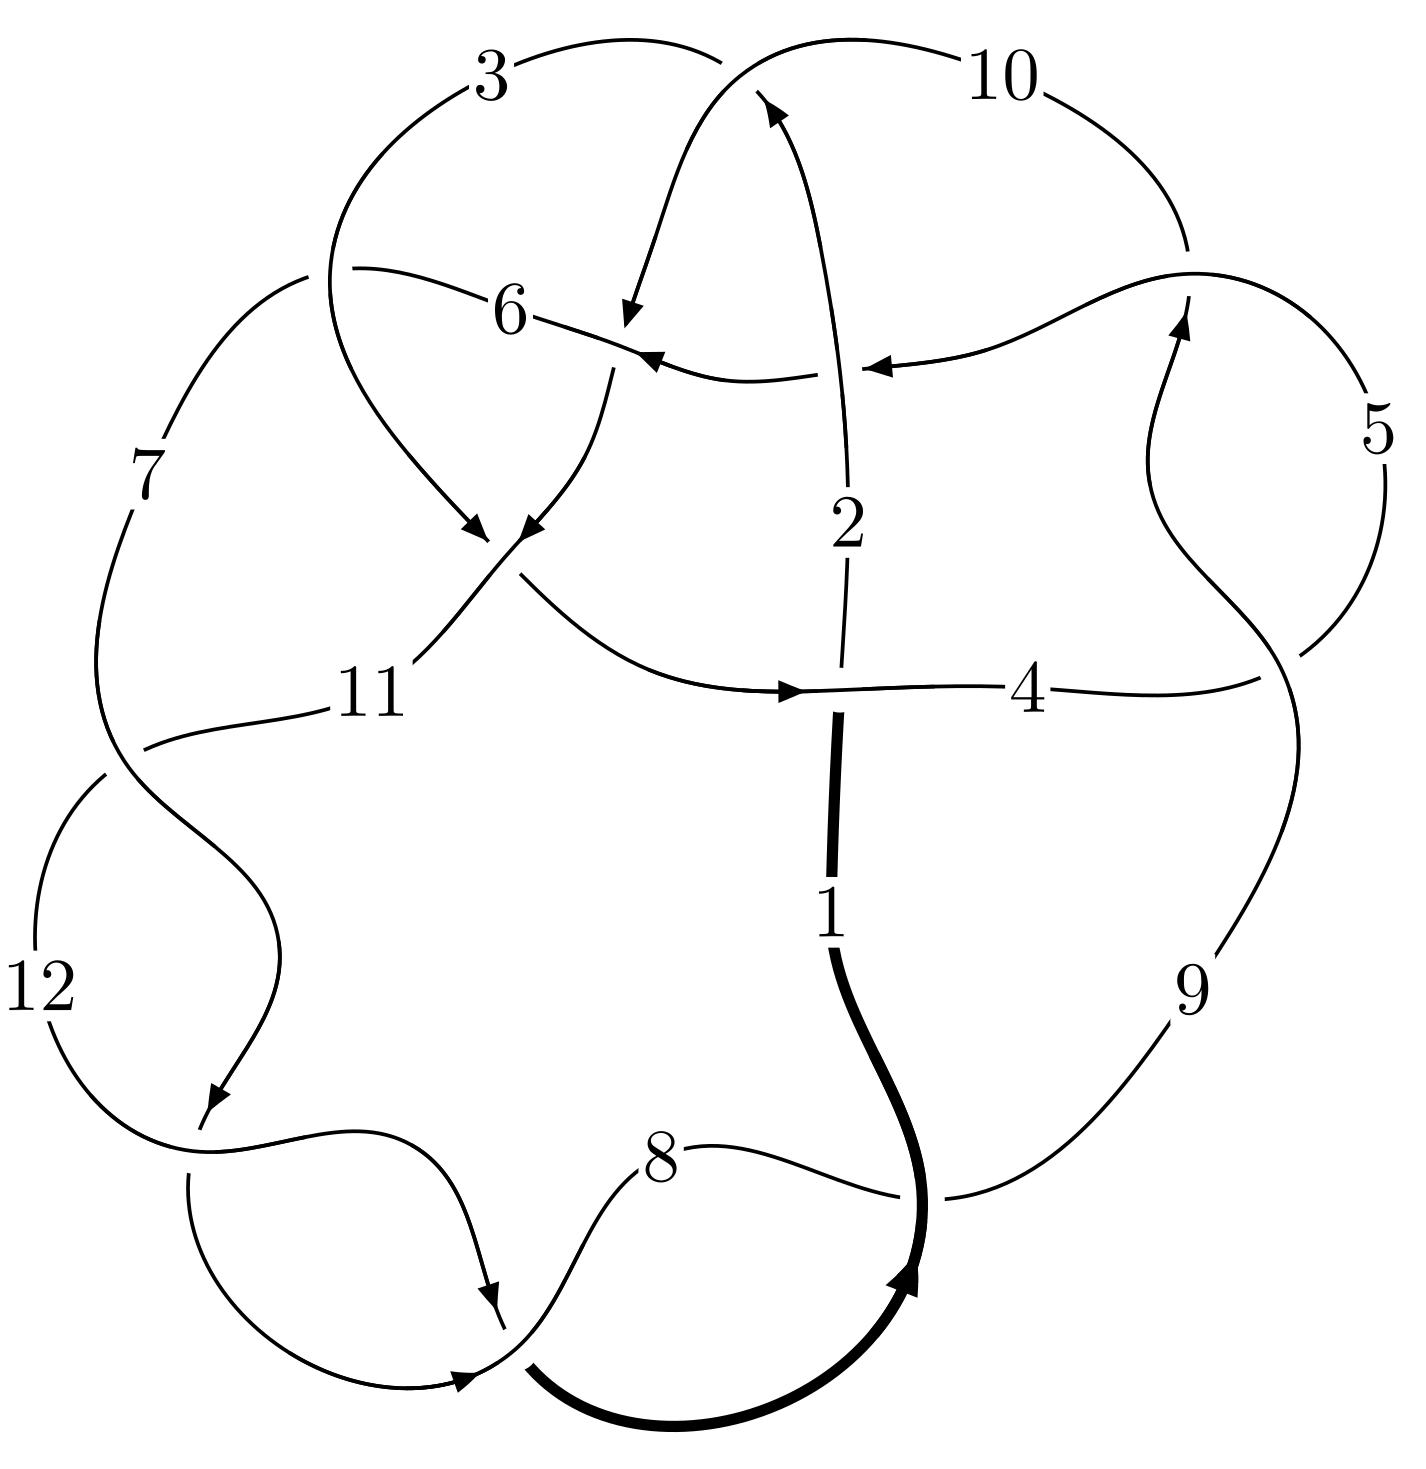
\includegraphics[width=112pt]{../../../GIT/diagram.site/Diagrams/png/1992_12a_1191.png}\\
\ \ \ A knot diagram\footnotemark}&
\allowdisplaybreaks
\textbf{Linearized knot diagam} \\
\cline{2-2}
 &
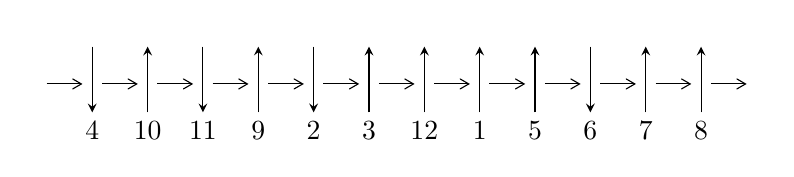
\begin{tikzpicture}[x=20pt, y=17pt]
	% nodes
	\node (C0) at (0, 0) {};
	\node (C1) at (1, 0) {};
	\node (C1U) at (1, +1) {};
	\node (C1D) at (1, -1) {4};

	\node (C2) at (2, 0) {};
	\node (C2U) at (2, +1) {};
	\node (C2D) at (2, -1) {10};

	\node (C3) at (3, 0) {};
	\node (C3U) at (3, +1) {};
	\node (C3D) at (3, -1) {11};

	\node (C4) at (4, 0) {};
	\node (C4U) at (4, +1) {};
	\node (C4D) at (4, -1) {9};

	\node (C5) at (5, 0) {};
	\node (C5U) at (5, +1) {};
	\node (C5D) at (5, -1) {2};

	\node (C6) at (6, 0) {};
	\node (C6U) at (6, +1) {};
	\node (C6D) at (6, -1) {3};

	\node (C7) at (7, 0) {};
	\node (C7U) at (7, +1) {};
	\node (C7D) at (7, -1) {12};

	\node (C8) at (8, 0) {};
	\node (C8U) at (8, +1) {};
	\node (C8D) at (8, -1) {1};

	\node (C9) at (9, 0) {};
	\node (C9U) at (9, +1) {};
	\node (C9D) at (9, -1) {5};

	\node (C10) at (10, 0) {};
	\node (C10U) at (10, +1) {};
	\node (C10D) at (10, -1) {6};

	\node (C11) at (11, 0) {};
	\node (C11U) at (11, +1) {};
	\node (C11D) at (11, -1) {7};

	\node (C12) at (12, 0) {};
	\node (C12U) at (12, +1) {};
	\node (C12D) at (12, -1) {8};
	\node (C13) at (13, 0) {};

	% arrows
	\draw[->,>={angle 60}]
	(C0) edge (C1) (C1) edge (C2) (C2) edge (C3) (C3) edge (C4) (C4) edge (C5) (C5) edge (C6) (C6) edge (C7) (C7) edge (C8) (C8) edge (C9) (C9) edge (C10) (C10) edge (C11) (C11) edge (C12) (C12) edge (C13) ;	\draw[->,>=stealth]
	(C1U) edge (C1D) (C2D) edge (C2U) (C3U) edge (C3D) (C4D) edge (C4U) (C5U) edge (C5D) (C6D) edge (C6U) (C7D) edge (C7U) (C8D) edge (C8U) (C9D) edge (C9U) (C10U) edge (C10D) (C11D) edge (C11U) (C12D) edge (C12U) ;
	\end{tikzpicture} \\
\hhline{~~} \\& 
\textbf{Solving Sequence} \\ \cline{2-2} 
 &
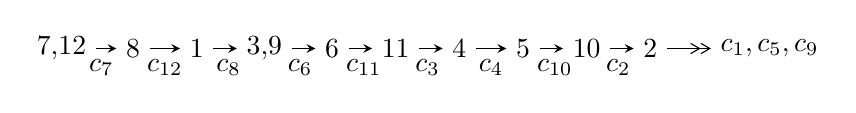
\begin{tikzpicture}[x=23pt, y=7pt]
	% node
	\node (A0) at (-1/8, 0) {7,12};
	\node (A1) at (1, 0) {8};
	\node (A2) at (2, 0) {1};
	\node (A3) at (49/16, 0) {3,9};
	\node (A4) at (33/8, 0) {6};
	\node (A5) at (41/8, 0) {11};
	\node (A6) at (49/8, 0) {4};
	\node (A7) at (57/8, 0) {5};
	\node (A8) at (65/8, 0) {10};
	\node (A9) at (73/8, 0) {2};
	\node (C1) at (1/2, -1) {$c_{7}$};
	\node (C2) at (3/2, -1) {$c_{12}$};
	\node (C3) at (5/2, -1) {$c_{8}$};
	\node (C4) at (29/8, -1) {$c_{6}$};
	\node (C5) at (37/8, -1) {$c_{11}$};
	\node (C6) at (45/8, -1) {$c_{3}$};
	\node (C7) at (53/8, -1) {$c_{4}$};
	\node (C8) at (61/8, -1) {$c_{10}$};
	\node (C9) at (69/8, -1) {$c_{2}$};
	\node (A10) at (11, 0) {$c_{1},c_{5},c_{9}$};

	% edge
	\draw[->,>=stealth]	
	(A0) edge (A1) (A1) edge (A2) (A2) edge (A3) (A3) edge (A4) (A4) edge (A5) (A5) edge (A6) (A6) edge (A7) (A7) edge (A8) (A8) edge (A9) ;
	\draw[->>,>={angle 60}]	
	(A9) edge (A10);
\end{tikzpicture} \\ 

\end{tabular} \\

\footnotetext{
The image of knot diagram is generated by the software ``\textbf{Draw programme}" developed by Andrew Bartholomew(\url{http://www.layer8.co.uk/maths/draw/index.htm\#Running-draw}), where we modified some parts for our purpose(\url{https://github.com/CATsTAILs/LinksPainter}).
}\phantom \\ \newline 
\centering \textbf{Ideals for irreducible components\footnotemark of $X_{\text{par}}$} 
 
\begin{align*}
I^u_{1}&=\langle 
4.36523\times10^{132} u^{90}-3.19353\times10^{132} u^{89}+\cdots+2.10482\times10^{131} b-5.51264\times10^{132},\\
\phantom{I^u_{1}}&\phantom{= \langle  }-1.18098\times10^{133} u^{90}+8.96992\times10^{132} u^{89}+\cdots+2.10482\times10^{131} a+1.66735\times10^{133},\\
\phantom{I^u_{1}}&\phantom{= \langle  }u^{91}-58 u^{89}+\cdots- u-1\rangle \\
I^u_{2}&=\langle 
- u^{13}+10 u^{11}-2 u^{10}-37 u^9+16 u^8+60 u^7-44 u^6-37 u^5+46 u^4+2 u^3-13 u^2+b+2 u+2,\\
\phantom{I^u_{2}}&\phantom{= \langle  }2 u^{13}- u^{12}-20 u^{11}+13 u^{10}+73 u^9-62 u^8-113 u^7+133 u^6+57 u^5-122 u^4+10 u^3+36 u^2+a-3 u-8,\\
\phantom{I^u_{2}}&\phantom{= \langle  }u^{14}-10 u^{12}+2 u^{11}+38 u^{10}-16 u^9-67 u^8+45 u^7+53 u^6-51 u^5-16 u^4+20 u^3+4 u^2-4 u-1\rangle \\
I^u_{3}&=\langle 
b,\;a+1,\;u+1\rangle \\
\\
\end{align*}
\raggedright * 3 irreducible components of $\dim_{\mathbb{C}}=0$, with total 106 representations.\\
\footnotetext{All coefficients of polynomials are rational numbers. But the coefficients are sometimes approximated in decimal forms when there is not enough margin.}
\newpage
\renewcommand{\arraystretch}{1}
\centering \section*{I. $I^u_{1}= \langle 4.37\times10^{132} u^{90}-3.19\times10^{132} u^{89}+\cdots+2.10\times10^{131} b-5.51\times10^{132},\;-1.18\times10^{133} u^{90}+8.97\times10^{132} u^{89}+\cdots+2.10\times10^{131} a+1.67\times10^{133},\;u^{91}-58 u^{89}+\cdots- u-1 \rangle$}
\flushleft \textbf{(i) Arc colorings}\\
\begin{tabular}{m{7pt} m{180pt} m{7pt} m{180pt} }
\flushright $a_{7}=$&$\begin{pmatrix}1\\0\end{pmatrix}$ \\
\flushright $a_{12}=$&$\begin{pmatrix}0\\u\end{pmatrix}$ \\
\flushright $a_{8}=$&$\begin{pmatrix}1\\- u^2\end{pmatrix}$ \\
\flushright $a_{1}=$&$\begin{pmatrix}u\\- u^3+u\end{pmatrix}$ \\
\flushright $a_{3}=$&$\begin{pmatrix}56.1084 u^{90}-42.6161 u^{89}+\cdots-50.0478 u-79.2156\\-20.7392 u^{90}+15.1725 u^{89}+\cdots-4.73282 u+26.1906\end{pmatrix}$ \\
\flushright $a_{9}=$&$\begin{pmatrix}- u^2+1\\u^4-2 u^2\end{pmatrix}$ \\
\flushright $a_{6}=$&$\begin{pmatrix}-56.8158 u^{90}+42.7041 u^{89}+\cdots-84.2527 u+77.3151\\20.4447 u^{90}-16.1446 u^{89}+\cdots+10.5300 u-28.4511\end{pmatrix}$ \\
\flushright $a_{11}=$&$\begin{pmatrix}- u\\u\end{pmatrix}$ \\
\flushright $a_{4}=$&$\begin{pmatrix}35.4678 u^{90}-27.0005 u^{89}+\cdots-57.9734 u-51.7720\\-0.0987024 u^{90}-0.443082 u^{89}+\cdots+3.19269 u-1.25306\end{pmatrix}$ \\
\flushright $a_{5}=$&$\begin{pmatrix}48.8252 u^{90}-36.5045 u^{89}+\cdots-52.0806 u-69.1683\\-25.0607 u^{90}+17.8324 u^{89}+\cdots-7.86324 u+31.3440\end{pmatrix}$ \\
\flushright $a_{10}=$&$\begin{pmatrix}-67.5498 u^{90}+50.1740 u^{89}+\cdots-9.65117 u+91.8368\\32.6880 u^{90}-23.5158 u^{89}+\cdots+17.8004 u-43.1141\end{pmatrix}$ \\
\flushright $a_{2}=$&$\begin{pmatrix}21.3595 u^{90}-17.2198 u^{89}+\cdots-78.0900 u-44.2105\\-0.0820261 u^{90}+1.41198 u^{89}+\cdots+0.825309 u+2.32895\end{pmatrix}$\\&\end{tabular}
\flushleft \textbf{(ii) Obstruction class $= -1$}\\~\\
\flushleft \textbf{(iii) Cusp Shapes $= -124.387 u^{90}+101.213 u^{89}+\cdots-117.598 u+140.246$}\\~\\
\newpage\renewcommand{\arraystretch}{1}
\flushleft \textbf{(iv) u-Polynomials at the component}\newline \\
\begin{tabular}{m{50pt}|m{274pt}}
Crossings & \hspace{64pt}u-Polynomials at each crossing \\
\hline $$\begin{aligned}c_{1}\end{aligned}$$&$\begin{aligned}
&u^{91}+26 u^{89}+\cdots+4521 u-1063
\end{aligned}$\\
\hline $$\begin{aligned}c_{2}\end{aligned}$$&$\begin{aligned}
&u^{91}+3 u^{90}+\cdots-107 u+47
\end{aligned}$\\
\hline $$\begin{aligned}c_{3}\end{aligned}$$&$\begin{aligned}
&u^{91}- u^{90}+\cdots-1664 u+256
\end{aligned}$\\
\hline $$\begin{aligned}c_{4},c_{9}\end{aligned}$$&$\begin{aligned}
&u^{91}- u^{90}+\cdots+40 u+16
\end{aligned}$\\
\hline $$\begin{aligned}c_{5}\end{aligned}$$&$\begin{aligned}
&u^{91}-2 u^{89}+\cdots-27 u+1
\end{aligned}$\\
\hline $$\begin{aligned}c_{6}\end{aligned}$$&$\begin{aligned}
&u^{91}-3 u^{90}+\cdots-20 u+478
\end{aligned}$\\
\hline $$\begin{aligned}c_{7},c_{8},c_{11}\\c_{12}\end{aligned}$$&$\begin{aligned}
&u^{91}-58 u^{89}+\cdots- u+1
\end{aligned}$\\
\hline $$\begin{aligned}c_{10}\end{aligned}$$&$\begin{aligned}
&u^{91}-4 u^{90}+\cdots+13 u+1
\end{aligned}$\\
\hline
\end{tabular}\\~\\
\newpage\renewcommand{\arraystretch}{1}
\flushleft \textbf{(v) Riley Polynomials at the component}\newline \\
\begin{tabular}{m{50pt}|m{274pt}}
Crossings & \hspace{64pt}Riley Polynomials at each crossing \\
\hline $$\begin{aligned}c_{1}\end{aligned}$$&$\begin{aligned}
&y^{91}+52 y^{90}+\cdots+271560435 y-1129969
\end{aligned}$\\
\hline $$\begin{aligned}c_{2}\end{aligned}$$&$\begin{aligned}
&y^{91}-27 y^{90}+\cdots+250585 y-2209
\end{aligned}$\\
\hline $$\begin{aligned}c_{3}\end{aligned}$$&$\begin{aligned}
&y^{91}+19 y^{90}+\cdots+638976 y-65536
\end{aligned}$\\
\hline $$\begin{aligned}c_{4},c_{9}\end{aligned}$$&$\begin{aligned}
&y^{91}-77 y^{90}+\cdots+20544 y-256
\end{aligned}$\\
\hline $$\begin{aligned}c_{5}\end{aligned}$$&$\begin{aligned}
&y^{91}-4 y^{90}+\cdots+43 y-1
\end{aligned}$\\
\hline $$\begin{aligned}c_{6}\end{aligned}$$&$\begin{aligned}
&y^{91}-33 y^{90}+\cdots+38548232 y-228484
\end{aligned}$\\
\hline $$\begin{aligned}c_{7},c_{8},c_{11}\\c_{12}\end{aligned}$$&$\begin{aligned}
&y^{91}-116 y^{90}+\cdots+183 y-1
\end{aligned}$\\
\hline $$\begin{aligned}c_{10}\end{aligned}$$&$\begin{aligned}
&y^{91}-14 y^{90}+\cdots+35 y-1
\end{aligned}$\\
\hline
\end{tabular}\\~\\
\newpage\flushleft \textbf{(vi) Complex Volumes and Cusp Shapes}
$$\begin{array}{c|c|c}  
\text{Solutions to }I^u_{1}& \I (\text{vol} + \sqrt{-1}CS) & \text{Cusp shape}\\
 \hline 
\begin{aligned}
u &= -0.917181 + 0.446358 I \\
a &= -0.350051 - 0.718722 I \\
b &= \phantom{-}0.752614 + 0.368141 I\end{aligned}
 & \phantom{-}1.10014 + 1.26315 I & \phantom{-0.000000 } 0 \\ \hline\begin{aligned}
u &= -0.917181 - 0.446358 I \\
a &= -0.350051 + 0.718722 I \\
b &= \phantom{-}0.752614 - 0.368141 I\end{aligned}
 & \phantom{-}1.10014 - 1.26315 I & \phantom{-0.000000 } 0 \\ \hline\begin{aligned}
u &= \phantom{-}1.020520 + 0.021459 I \\
a &= \phantom{-}1.65965 + 0.12252 I \\
b &= -1.274710 + 0.013134 I\end{aligned}
 & \phantom{-}6.37995 - 0.00443 I & \phantom{-0.000000 } 0 \\ \hline\begin{aligned}
u &= \phantom{-}1.020520 - 0.021459 I \\
a &= \phantom{-}1.65965 - 0.12252 I \\
b &= -1.274710 - 0.013134 I\end{aligned}
 & \phantom{-}6.37995 + 0.00443 I & \phantom{-0.000000 } 0 \\ \hline\begin{aligned}
u &= \phantom{-}0.912677 + 0.338207 I \\
a &= \phantom{-}1.087310 - 0.365705 I \\
b &= -0.672974 - 0.988089 I\end{aligned}
 & \phantom{-}2.76497 + 5.71335 I & \phantom{-0.000000 } 0 \\ \hline\begin{aligned}
u &= \phantom{-}0.912677 - 0.338207 I \\
a &= \phantom{-}1.087310 + 0.365705 I \\
b &= -0.672974 + 0.988089 I\end{aligned}
 & \phantom{-}2.76497 - 5.71335 I & \phantom{-0.000000 } 0 \\ \hline\begin{aligned}
u &= \phantom{-}0.842246 + 0.427903 I \\
a &= -1.57000 + 0.86044 I \\
b &= \phantom{-}1.137440 + 0.719196 I\end{aligned}
 & \phantom{-}0.83657 + 8.60958 I & \phantom{-0.000000 } 0 \\ \hline\begin{aligned}
u &= \phantom{-}0.842246 - 0.427903 I \\
a &= -1.57000 - 0.86044 I \\
b &= \phantom{-}1.137440 - 0.719196 I\end{aligned}
 & \phantom{-}0.83657 - 8.60958 I & \phantom{-0.000000 } 0 \\ \hline\begin{aligned}
u &= -0.049155 + 0.925373 I \\
a &= -0.018450 - 0.240418 I \\
b &= \phantom{-}0.787113 + 0.434682 I\end{aligned}
 & \phantom{-}4.35215 - 0.70387 I & \phantom{-0.000000 } 0 \\ \hline\begin{aligned}
u &= -0.049155 - 0.925373 I \\
a &= -0.018450 + 0.240418 I \\
b &= \phantom{-}0.787113 - 0.434682 I\end{aligned}
 & \phantom{-}4.35215 + 0.70387 I & \phantom{-0.000000 } 0\\
 \hline 
 \end{array}$$\newpage$$\begin{array}{c|c|c}  
\text{Solutions to }I^u_{1}& \I (\text{vol} + \sqrt{-1}CS) & \text{Cusp shape}\\
 \hline 
\begin{aligned}
u &= \phantom{-}0.909377 + 0.121317 I \\
a &= -1.74806 - 1.51726 I \\
b &= \phantom{-}0.656466 + 0.156356 I\end{aligned}
 & \phantom{-}6.80329 + 5.85078 I & \phantom{-0.000000 } 0 \\ \hline\begin{aligned}
u &= \phantom{-}0.909377 - 0.121317 I \\
a &= -1.74806 + 1.51726 I \\
b &= \phantom{-}0.656466 - 0.156356 I\end{aligned}
 & \phantom{-}6.80329 - 5.85078 I & \phantom{-0.000000 } 0 \\ \hline\begin{aligned}
u &= -0.855576 + 0.198161 I \\
a &= -1.69427 - 0.84476 I \\
b &= \phantom{-}0.600470 - 0.528724 I\end{aligned}
 & \phantom{-}0.41511 - 1.73319 I & \phantom{-0.000000 } 0 \\ \hline\begin{aligned}
u &= -0.855576 - 0.198161 I \\
a &= -1.69427 + 0.84476 I \\
b &= \phantom{-}0.600470 + 0.528724 I\end{aligned}
 & \phantom{-}0.41511 + 1.73319 I & \phantom{-0.000000 } 0 \\ \hline\begin{aligned}
u &= \phantom{-}0.170636 + 0.858640 I \\
a &= \phantom{-}0.270440 - 0.217975 I \\
b &= -0.988141 - 0.796603 I\end{aligned}
 & \phantom{-}2.60854 + 9.24166 I & \phantom{-0.000000 } 0 \\ \hline\begin{aligned}
u &= \phantom{-}0.170636 - 0.858640 I \\
a &= \phantom{-}0.270440 + 0.217975 I \\
b &= -0.988141 + 0.796603 I\end{aligned}
 & \phantom{-}2.60854 - 9.24166 I & \phantom{-0.000000 } 0 \\ \hline\begin{aligned}
u &= \phantom{-}0.798624 + 0.317069 I \\
a &= \phantom{-}1.49211 - 0.38463 I \\
b &= -1.13354 - 0.85618 I\end{aligned}
 & \phantom{-}2.71888 + 4.11027 I & \phantom{-0.000000 } 0 \\ \hline\begin{aligned}
u &= \phantom{-}0.798624 - 0.317069 I \\
a &= \phantom{-}1.49211 + 0.38463 I \\
b &= -1.13354 + 0.85618 I\end{aligned}
 & \phantom{-}2.71888 - 4.11027 I & \phantom{-0.000000 } 0 \\ \hline\begin{aligned}
u &= -0.958558 + 0.619174 I \\
a &= -1.304190 - 0.198758 I \\
b &= \phantom{-}1.190730 - 0.754942 I\end{aligned}
 & \phantom{-}7.19572 - 4.42968 I & \phantom{-0.000000 } 0 \\ \hline\begin{aligned}
u &= -0.958558 - 0.619174 I \\
a &= -1.304190 + 0.198758 I \\
b &= \phantom{-}1.190730 + 0.754942 I\end{aligned}
 & \phantom{-}7.19572 + 4.42968 I & \phantom{-0.000000 } 0\\
 \hline 
 \end{array}$$\newpage$$\begin{array}{c|c|c}  
\text{Solutions to }I^u_{1}& \I (\text{vol} + \sqrt{-1}CS) & \text{Cusp shape}\\
 \hline 
\begin{aligned}
u &= -1.010410 + 0.532785 I \\
a &= \phantom{-}1.63192 + 0.38601 I \\
b &= -1.26642 + 0.85939 I\end{aligned}
 & \phantom{-}6.2099 - 13.8413 I & \phantom{-0.000000 } 0 \\ \hline\begin{aligned}
u &= -1.010410 - 0.532785 I \\
a &= \phantom{-}1.63192 - 0.38601 I \\
b &= -1.26642 - 0.85939 I\end{aligned}
 & \phantom{-}6.2099 + 13.8413 I & \phantom{-0.000000 } 0 \\ \hline\begin{aligned}
u &= \phantom{-}1.012830 + 0.547009 I \\
a &= -0.666318 + 0.854147 I \\
b &= \phantom{-}0.845873 + 0.040235 I\end{aligned}
 & \phantom{-}7.74795 + 5.61965 I & \phantom{-0.000000 } 0 \\ \hline\begin{aligned}
u &= \phantom{-}1.012830 - 0.547009 I \\
a &= -0.666318 - 0.854147 I \\
b &= \phantom{-}0.845873 - 0.040235 I\end{aligned}
 & \phantom{-}7.74795 - 5.61965 I & \phantom{-0.000000 } 0 \\ \hline\begin{aligned}
u &= \phantom{-}1.158320 + 0.061570 I \\
a &= \phantom{-}2.09123 + 0.11464 I \\
b &= -1.43859 - 0.11203 I\end{aligned}
 & \phantom{-}6.35878 - 0.00374 I & \phantom{-0.000000 } 0 \\ \hline\begin{aligned}
u &= \phantom{-}1.158320 - 0.061570 I \\
a &= \phantom{-}2.09123 - 0.11464 I \\
b &= -1.43859 + 0.11203 I\end{aligned}
 & \phantom{-}6.35878 + 0.00374 I & \phantom{-0.000000 } 0 \\ \hline\begin{aligned}
u &= -0.827706 + 0.023758 I \\
a &= -1.94653 - 0.03034 I \\
b &= \phantom{-}1.30788 + 1.14736 I\end{aligned}
 & \phantom{-}5.75955 + 4.36365 I & \phantom{-0.000000 } 0 \\ \hline\begin{aligned}
u &= -0.827706 - 0.023758 I \\
a &= -1.94653 + 0.03034 I \\
b &= \phantom{-}1.30788 - 1.14736 I\end{aligned}
 & \phantom{-}5.75955 - 4.36365 I & \phantom{-0.000000 } 0 \\ \hline\begin{aligned}
u &= \phantom{-}1.20776\phantom{ +0.000000I} \\
a &= \phantom{-}1.23537\phantom{ +0.000000I} \\
b &= -0.150179\phantom{ +0.000000I}\end{aligned}
 & \phantom{-}1.50241\phantom{ +0.000000I} & \phantom{-0.000000 } 0 \\ \hline\begin{aligned}
u &= -0.692576 + 0.369176 I \\
a &= -0.252568 + 1.293030 I \\
b &= -0.15549 - 1.61967 I\end{aligned}
 & \phantom{-}3.29248 - 5.87120 I & \phantom{-0.000000 } 0\\
 \hline 
 \end{array}$$\newpage$$\begin{array}{c|c|c}  
\text{Solutions to }I^u_{1}& \I (\text{vol} + \sqrt{-1}CS) & \text{Cusp shape}\\
 \hline 
\begin{aligned}
u &= -0.692576 - 0.369176 I \\
a &= -0.252568 - 1.293030 I \\
b &= -0.15549 + 1.61967 I\end{aligned}
 & \phantom{-}3.29248 + 5.87120 I & \phantom{-0.000000 } 0 \\ \hline\begin{aligned}
u &= \phantom{-}0.871395 + 0.870623 I \\
a &= \phantom{-}0.199766 - 0.694070 I \\
b &= -0.701199 + 0.494745 I\end{aligned}
 & \phantom{-}4.43105 - 3.66394 I & \phantom{-0.000000 } 0 \\ \hline\begin{aligned}
u &= \phantom{-}0.871395 - 0.870623 I \\
a &= \phantom{-}0.199766 + 0.694070 I \\
b &= -0.701199 - 0.494745 I\end{aligned}
 & \phantom{-}4.43105 + 3.66394 I & \phantom{-0.000000 } 0 \\ \hline\begin{aligned}
u &= -0.752182\phantom{ +0.000000I} \\
a &= \phantom{-}3.63130\phantom{ +0.000000I} \\
b &= -1.36493\phantom{ +0.000000I}\end{aligned}
 & \phantom{-}3.54118\phantom{ +0.000000I} & \phantom{-0.000000 } 0 \\ \hline\begin{aligned}
u &= -0.741016\phantom{ +0.000000I} \\
a &= -0.850183\phantom{ +0.000000I} \\
b &= \phantom{-}0.113569\phantom{ +0.000000I}\end{aligned}
 & \phantom{-}1.10828\phantom{ +0.000000I} & \phantom{-0.000000 } 0 \\ \hline\begin{aligned}
u &= -0.695366 + 0.186808 I \\
a &= \phantom{-}0.35620 + 2.27599 I \\
b &= -0.784084 + 0.061653 I\end{aligned}
 & \phantom{-}2.27067 - 0.45074 I & \phantom{-0.000000 } 0 \\ \hline\begin{aligned}
u &= -0.695366 - 0.186808 I \\
a &= \phantom{-}0.35620 - 2.27599 I \\
b &= -0.784084 - 0.061653 I\end{aligned}
 & \phantom{-}2.27067 + 0.45074 I & \phantom{-0.000000 } 0 \\ \hline\begin{aligned}
u &= -0.628840 + 0.325941 I \\
a &= -0.679726 + 0.307313 I \\
b &= -0.344482 - 0.126930 I\end{aligned}
 & \phantom{-}1.371510 - 0.206959 I & \phantom{-0.000000 } 0 \\ \hline\begin{aligned}
u &= -0.628840 - 0.325941 I \\
a &= -0.679726 - 0.307313 I \\
b &= -0.344482 + 0.126930 I\end{aligned}
 & \phantom{-}1.371510 + 0.206959 I & \phantom{-0.000000 } 0 \\ \hline\begin{aligned}
u &= \phantom{-}0.601513 + 0.261883 I \\
a &= \phantom{-}0.143854 + 0.590721 I \\
b &= \phantom{-}0.441427 - 1.013250 I\end{aligned}
 & -1.19187 + 2.41953 I & \phantom{-0.000000 } 0. - 7.66477 I\\
 \hline 
 \end{array}$$\newpage$$\begin{array}{c|c|c}  
\text{Solutions to }I^u_{1}& \I (\text{vol} + \sqrt{-1}CS) & \text{Cusp shape}\\
 \hline 
\begin{aligned}
u &= \phantom{-}0.601513 - 0.261883 I \\
a &= \phantom{-}0.143854 - 0.590721 I \\
b &= \phantom{-}0.441427 + 1.013250 I\end{aligned}
 & -1.19187 - 2.41953 I & \phantom{-0.000000 -}0. + 7.66477 I \\ \hline\begin{aligned}
u &= \phantom{-}0.014121 + 0.652849 I \\
a &= \phantom{-}0.247154 - 0.479642 I \\
b &= \phantom{-}0.943310 - 0.640973 I\end{aligned}
 & -1.67591 - 4.97592 I & \phantom{-}4.00000 + 6.22523 I \\ \hline\begin{aligned}
u &= \phantom{-}0.014121 - 0.652849 I \\
a &= \phantom{-}0.247154 + 0.479642 I \\
b &= \phantom{-}0.943310 + 0.640973 I\end{aligned}
 & -1.67591 + 4.97592 I & \phantom{-}4.00000 - 6.22523 I \\ \hline\begin{aligned}
u &= -0.228822 + 0.569931 I \\
a &= \phantom{-}1.242050 - 0.011593 I \\
b &= -0.792425 + 1.135470 I\end{aligned}
 & \phantom{-}1.91858 + 2.59973 I & \phantom{-}2.55627 - 3.29477 I \\ \hline\begin{aligned}
u &= -0.228822 - 0.569931 I \\
a &= \phantom{-}1.242050 + 0.011593 I \\
b &= -0.792425 - 1.135470 I\end{aligned}
 & \phantom{-}1.91858 - 2.59973 I & \phantom{-}2.55627 + 3.29477 I \\ \hline\begin{aligned}
u &= -0.094291 + 0.541879 I \\
a &= -0.557308 + 1.003780 I \\
b &= -0.455963 + 0.707318 I\end{aligned}
 & -0.30212 - 2.71649 I & \phantom{-}1.16599 + 6.03643 I \\ \hline\begin{aligned}
u &= -0.094291 - 0.541879 I \\
a &= -0.557308 - 1.003780 I \\
b &= -0.455963 - 0.707318 I\end{aligned}
 & -0.30212 + 2.71649 I & \phantom{-}1.16599 - 6.03643 I \\ \hline\begin{aligned}
u &= -1.49316\phantom{ +0.000000I} \\
a &= -2.56595\phantom{ +0.000000I} \\
b &= \phantom{-}1.76633\phantom{ +0.000000I}\end{aligned}
 & \phantom{-}3.30274\phantom{ +0.000000I} & \phantom{-0.000000 } 0 \\ \hline\begin{aligned}
u &= -0.001188 + 0.400466 I \\
a &= -1.271860 + 0.075004 I \\
b &= -0.674817 + 0.552835 I\end{aligned}
 & \phantom{-}0.43902 - 1.57022 I & \phantom{-}4.00266 + 2.96421 I \\ \hline\begin{aligned}
u &= -0.001188 - 0.400466 I \\
a &= -1.271860 - 0.075004 I \\
b &= -0.674817 - 0.552835 I\end{aligned}
 & \phantom{-}0.43902 + 1.57022 I & \phantom{-}4.00266 - 2.96421 I\\
 \hline 
 \end{array}$$\newpage$$\begin{array}{c|c|c}  
\text{Solutions to }I^u_{1}& \I (\text{vol} + \sqrt{-1}CS) & \text{Cusp shape}\\
 \hline 
\begin{aligned}
u &= -1.60395 + 0.03130 I \\
a &= -0.211427 - 1.129280 I \\
b &= \phantom{-}0.29839 + 1.45886 I\end{aligned}
 & \phantom{-}6.43796 - 3.26756 I & \phantom{-0.000000 } 0 \\ \hline\begin{aligned}
u &= -1.60395 - 0.03130 I \\
a &= -0.211427 + 1.129280 I \\
b &= \phantom{-}0.29839 - 1.45886 I\end{aligned}
 & \phantom{-}6.43796 + 3.26756 I & \phantom{-0.000000 } 0 \\ \hline\begin{aligned}
u &= \phantom{-}1.61544 + 0.08861 I \\
a &= \phantom{-}0.184899 + 0.051274 I \\
b &= -0.407141 - 0.545139 I\end{aligned}
 & \phantom{-}9.04789 + 1.72598 I & \phantom{-0.000000 } 0 \\ \hline\begin{aligned}
u &= \phantom{-}1.61544 - 0.08861 I \\
a &= \phantom{-}0.184899 - 0.051274 I \\
b &= -0.407141 + 0.545139 I\end{aligned}
 & \phantom{-}9.04789 - 1.72598 I & \phantom{-0.000000 } 0 \\ \hline\begin{aligned}
u &= \phantom{-}0.141849 + 0.347474 I \\
a &= -1.10267 + 2.06537 I \\
b &= \phantom{-}0.641497 + 0.536873 I\end{aligned}
 & -2.40242 - 0.11800 I & -5.09885 - 1.12207 I \\ \hline\begin{aligned}
u &= \phantom{-}0.141849 - 0.347474 I \\
a &= -1.10267 - 2.06537 I \\
b &= \phantom{-}0.641497 - 0.536873 I\end{aligned}
 & -2.40242 + 0.11800 I & -5.09885 + 1.12207 I \\ \hline\begin{aligned}
u &= \phantom{-}1.63813 + 0.08293 I \\
a &= -0.15558 - 1.84572 I \\
b &= \phantom{-}0.06614 + 2.09277 I\end{aligned}
 & \phantom{-}11.43140 + 7.43619 I & \phantom{-0.000000 } 0 \\ \hline\begin{aligned}
u &= \phantom{-}1.63813 - 0.08293 I \\
a &= -0.15558 + 1.84572 I \\
b &= \phantom{-}0.06614 - 2.09277 I\end{aligned}
 & \phantom{-}11.43140 - 7.43619 I & \phantom{-0.000000 } 0 \\ \hline\begin{aligned}
u &= \phantom{-}1.64405 + 0.03849 I \\
a &= \phantom{-}1.38387 - 1.09007 I \\
b &= -0.893959 - 0.323763 I\end{aligned}
 & \phantom{-}10.54520 + 1.19802 I & \phantom{-0.000000 } 0 \\ \hline\begin{aligned}
u &= \phantom{-}1.64405 - 0.03849 I \\
a &= \phantom{-}1.38387 + 1.09007 I \\
b &= -0.893959 + 0.323763 I\end{aligned}
 & \phantom{-}10.54520 - 1.19802 I & \phantom{-0.000000 } 0\\
 \hline 
 \end{array}$$\newpage$$\begin{array}{c|c|c}  
\text{Solutions to }I^u_{1}& \I (\text{vol} + \sqrt{-1}CS) & \text{Cusp shape}\\
 \hline 
\begin{aligned}
u &= \phantom{-}1.65603\phantom{ +0.000000I} \\
a &= \phantom{-}2.84891\phantom{ +0.000000I} \\
b &= -1.56819\phantom{ +0.000000I}\end{aligned}
 & \phantom{-}12.0821\phantom{ +0.000000I} & \phantom{-0.000000 } 0 \\ \hline\begin{aligned}
u &= -1.65904 + 0.08425 I \\
a &= \phantom{-}1.99380 - 0.30053 I \\
b &= -1.45706 + 0.97395 I\end{aligned}
 & \phantom{-}11.30970 - 5.62963 I & \phantom{-0.000000 } 0 \\ \hline\begin{aligned}
u &= -1.65904 - 0.08425 I \\
a &= \phantom{-}1.99380 + 0.30053 I \\
b &= -1.45706 - 0.97395 I\end{aligned}
 & \phantom{-}11.30970 + 5.62963 I & \phantom{-0.000000 } 0 \\ \hline\begin{aligned}
u &= -1.66431 + 0.10950 I \\
a &= -2.01278 - 0.18168 I \\
b &= \phantom{-}1.29842 - 0.76043 I\end{aligned}
 & \phantom{-}9.5241 - 10.6370 I & \phantom{-0.000000 } 0 \\ \hline\begin{aligned}
u &= -1.66431 - 0.10950 I \\
a &= -2.01278 + 0.18168 I \\
b &= \phantom{-}1.29842 + 0.76043 I\end{aligned}
 & \phantom{-}9.5241 + 10.6370 I & \phantom{-0.000000 } 0 \\ \hline\begin{aligned}
u &= -0.327010 + 0.024834 I \\
a &= -2.45501 + 0.42707 I \\
b &= -1.050700 - 0.022615 I\end{aligned}
 & \phantom{-}2.25017 - 0.00521 I & \phantom{-}25.7179 - 12.5088 I \\ \hline\begin{aligned}
u &= -0.327010 - 0.024834 I \\
a &= -2.45501 - 0.42707 I \\
b &= -1.050700 + 0.022615 I\end{aligned}
 & \phantom{-}2.25017 + 0.00521 I & \phantom{-}25.7179 + 12.5088 I \\ \hline\begin{aligned}
u &= \phantom{-}1.67382 + 0.00252 I \\
a &= -2.09500 + 0.64314 I \\
b &= \phantom{-}1.60216 - 1.26474 I\end{aligned}
 & \phantom{-}14.6420 - 4.2859 I & \phantom{-0.000000 } 0 \\ \hline\begin{aligned}
u &= \phantom{-}1.67382 - 0.00252 I \\
a &= -2.09500 - 0.64314 I \\
b &= \phantom{-}1.60216 + 1.26474 I\end{aligned}
 & \phantom{-}14.6420 + 4.2859 I & \phantom{-0.000000 } 0 \\ \hline\begin{aligned}
u &= \phantom{-}1.67890 + 0.04717 I \\
a &= -1.60010 + 0.25978 I \\
b &= \phantom{-}0.760804 + 0.612967 I\end{aligned}
 & \phantom{-}9.37397 + 2.64843 I & \phantom{-0.000000 } 0\\
 \hline 
 \end{array}$$\newpage$$\begin{array}{c|c|c}  
\text{Solutions to }I^u_{1}& \I (\text{vol} + \sqrt{-1}CS) & \text{Cusp shape}\\
 \hline 
\begin{aligned}
u &= \phantom{-}1.67890 - 0.04717 I \\
a &= -1.60010 - 0.25978 I \\
b &= \phantom{-}0.760804 - 0.612967 I\end{aligned}
 & \phantom{-}9.37397 - 2.64843 I & \phantom{-0.000000 } 0 \\ \hline\begin{aligned}
u &= -1.68883 + 0.03116 I \\
a &= -1.46816 + 0.84245 I \\
b &= \phantom{-}0.733381 + 0.158115 I\end{aligned}
 & \phantom{-}16.0083 - 6.4456 I & \phantom{-0.000000 } 0 \\ \hline\begin{aligned}
u &= -1.68883 - 0.03116 I \\
a &= -1.46816 - 0.84245 I \\
b &= \phantom{-}0.733381 - 0.158115 I\end{aligned}
 & \phantom{-}16.0083 + 6.4456 I & \phantom{-0.000000 } 0 \\ \hline\begin{aligned}
u &= -1.69089 + 0.08739 I \\
a &= \phantom{-}1.263860 - 0.324673 I \\
b &= -0.81079 + 1.19205 I\end{aligned}
 & \phantom{-}11.91300 - 7.36719 I & \phantom{-0.000000 } 0 \\ \hline\begin{aligned}
u &= -1.69089 - 0.08739 I \\
a &= \phantom{-}1.263860 + 0.324673 I \\
b &= -0.81079 - 1.19205 I\end{aligned}
 & \phantom{-}11.91300 + 7.36719 I & \phantom{-0.000000 } 0 \\ \hline\begin{aligned}
u &= \phantom{-}1.69395 + 0.07536 I \\
a &= -1.185220 + 0.193629 I \\
b &= \phantom{-}0.839978 + 0.209950 I\end{aligned}
 & \phantom{-}10.47930 + 0.62266 I & \phantom{-0.000000 } 0 \\ \hline\begin{aligned}
u &= \phantom{-}1.69395 - 0.07536 I \\
a &= -1.185220 - 0.193629 I \\
b &= \phantom{-}0.839978 - 0.209950 I\end{aligned}
 & \phantom{-}10.47930 - 0.62266 I & \phantom{-0.000000 } 0 \\ \hline\begin{aligned}
u &= -1.70284 + 0.02337 I \\
a &= \phantom{-}1.79568 - 0.24863 I \\
b &= -1.170090 - 0.204979 I\end{aligned}
 & \phantom{-}16.0167 - 0.3960 I & \phantom{-0.000000 } 0 \\ \hline\begin{aligned}
u &= -1.70284 - 0.02337 I \\
a &= \phantom{-}1.79568 + 0.24863 I \\
b &= -1.170090 + 0.204979 I\end{aligned}
 & \phantom{-}16.0167 + 0.3960 I & \phantom{-0.000000 } 0 \\ \hline\begin{aligned}
u &= -1.71287\phantom{ +0.000000I} \\
a &= \phantom{-}1.96336\phantom{ +0.000000I} \\
b &= -1.57408\phantom{ +0.000000I}\end{aligned}
 & \phantom{-}16.0925\phantom{ +0.000000I} & \phantom{-0.000000 } 0\\
 \hline 
 \end{array}$$\newpage$$\begin{array}{c|c|c}  
\text{Solutions to }I^u_{1}& \I (\text{vol} + \sqrt{-1}CS) & \text{Cusp shape}\\
 \hline 
\begin{aligned}
u &= \phantom{-}1.70600 + 0.17492 I \\
a &= -2.06447 - 0.11832 I \\
b &= \phantom{-}1.53935 + 0.77519 I\end{aligned}
 & \phantom{-}16.3686 + 7.5807 I & \phantom{-0.000000 } 0 \\ \hline\begin{aligned}
u &= \phantom{-}1.70600 - 0.17492 I \\
a &= -2.06447 + 0.11832 I \\
b &= \phantom{-}1.53935 - 0.77519 I\end{aligned}
 & \phantom{-}16.3686 - 7.5807 I & \phantom{-0.000000 } 0 \\ \hline\begin{aligned}
u &= -1.71338 + 0.14789 I \\
a &= -1.251830 - 0.547436 I \\
b &= \phantom{-}1.002740 - 0.286277 I\end{aligned}
 & \phantom{-}17.1980 - 8.3922 I & \phantom{-0.000000 } 0 \\ \hline\begin{aligned}
u &= -1.71338 - 0.14789 I \\
a &= -1.251830 + 0.547436 I \\
b &= \phantom{-}1.002740 + 0.286277 I\end{aligned}
 & \phantom{-}17.1980 + 8.3922 I & \phantom{-0.000000 } 0 \\ \hline\begin{aligned}
u &= \phantom{-}1.71531 + 0.15107 I \\
a &= \phantom{-}2.11203 + 0.06014 I \\
b &= -1.46699 - 0.87443 I\end{aligned}
 & \phantom{-}15.6677 + 16.6133 I & \phantom{-0.000000 } 0 \\ \hline\begin{aligned}
u &= \phantom{-}1.71531 - 0.15107 I \\
a &= \phantom{-}2.11203 - 0.06014 I \\
b &= -1.46699 + 0.87443 I\end{aligned}
 & \phantom{-}15.6677 - 16.6133 I & \phantom{-0.000000 } 0 \\ \hline\begin{aligned}
u &= -0.118525 + 0.147072 I \\
a &= -5.10070 + 3.31269 I \\
b &= \phantom{-}0.784408 - 0.784768 I\end{aligned}
 & \phantom{-}3.62366 - 4.82368 I & \phantom{-}8.27128 + 5.35281 I \\ \hline\begin{aligned}
u &= -0.118525 - 0.147072 I \\
a &= -5.10070 - 3.31269 I \\
b &= \phantom{-}0.784408 + 0.784768 I\end{aligned}
 & \phantom{-}3.62366 + 4.82368 I & \phantom{-}8.27128 - 5.35281 I \\ \hline\begin{aligned}
u &= -1.81169 + 0.19062 I \\
a &= \phantom{-}0.936030 + 0.424848 I \\
b &= -0.702838 + 0.003311 I\end{aligned}
 & \phantom{-}14.02360 - 1.03329 I & \phantom{-0.000000 } 0 \\ \hline\begin{aligned}
u &= -1.81169 - 0.19062 I \\
a &= \phantom{-}0.936030 - 0.424848 I \\
b &= -0.702838 - 0.003311 I\end{aligned}
 & \phantom{-}14.02360 + 1.03329 I & \phantom{-0.000000 } 0\\
 \hline 
 \end{array}$$\newpage$$\begin{array}{c|c|c}  
\text{Solutions to }I^u_{1}& \I (\text{vol} + \sqrt{-1}CS) & \text{Cusp shape}\\
 \hline 
\begin{aligned}
u &= \phantom{-}0.0762493\phantom{ +0.000000I} \\
a &= -16.9219\phantom{ +0.000000I} \\
b &= \phantom{-}0.601126\phantom{ +0.000000I}\end{aligned}
 & -2.56020\phantom{ +0.000000I} & -18.0060\phantom{ +0.000000I}\\
 \hline 
 \end{array}$$\newpage\newpage\renewcommand{\arraystretch}{1}
\centering \section*{II. $I^u_{2}= \langle - u^{13}+10 u^{11}+\cdots+b+2,\;2 u^{13}- u^{12}+\cdots+a-8,\;u^{14}-10 u^{12}+\cdots-4 u-1 \rangle$}
\flushleft \textbf{(i) Arc colorings}\\
\begin{tabular}{m{7pt} m{180pt} m{7pt} m{180pt} }
\flushright $a_{7}=$&$\begin{pmatrix}1\\0\end{pmatrix}$ \\
\flushright $a_{12}=$&$\begin{pmatrix}0\\u\end{pmatrix}$ \\
\flushright $a_{8}=$&$\begin{pmatrix}1\\- u^2\end{pmatrix}$ \\
\flushright $a_{1}=$&$\begin{pmatrix}u\\- u^3+u\end{pmatrix}$ \\
\flushright $a_{3}=$&$\begin{pmatrix}-2 u^{13}+u^{12}+\cdots+3 u+8\\u^{13}-10 u^{11}+\cdots-2 u-2\end{pmatrix}$ \\
\flushright $a_{9}=$&$\begin{pmatrix}- u^2+1\\u^4-2 u^2\end{pmatrix}$ \\
\flushright $a_{6}=$&$\begin{pmatrix}2 u^{13}-21 u^{11}+\cdots-5 u-7\\- u^{12}+u^{11}+\cdots-6 u-1\end{pmatrix}$ \\
\flushright $a_{11}=$&$\begin{pmatrix}- u\\u\end{pmatrix}$ \\
\flushright $a_{4}=$&$\begin{pmatrix}-2 u^{13}+20 u^{11}+\cdots-34 u^2+7\\u^{13}+u^{12}+\cdots+u-1\end{pmatrix}$ \\
\flushright $a_{5}=$&$\begin{pmatrix}-2 u^{13}+20 u^{11}+\cdots-4 u+6\\u^{13}-10 u^{11}+\cdots+u-1\end{pmatrix}$ \\
\flushright $a_{10}=$&$\begin{pmatrix}u^{10}- u^9-7 u^8+9 u^7+14 u^6-26 u^5-2 u^4+24 u^3-12 u^2\\u^{11}- u^{10}+\cdots+4 u+2\end{pmatrix}$ \\
\flushright $a_{2}=$&$\begin{pmatrix}-3 u^{13}+u^{12}+\cdots+7 u+12\\u^{10}- u^9-7 u^8+7 u^7+16 u^6-16 u^5-13 u^4+14 u^3+3 u^2-5 u-2\end{pmatrix}$\\&\end{tabular}
\flushleft \textbf{(ii) Obstruction class $= 1$}\\~\\
\flushleft \textbf{(iii) Cusp Shapes $= 10 u^{13}-98 u^{11}+26 u^{10}+356 u^9-202 u^8-553 u^7+532 u^6+258 u^5-504 u^4+116 u^3+78 u^2-41 u+16$}\\~\\
\newpage\renewcommand{\arraystretch}{1}
\flushleft \textbf{(iv) u-Polynomials at the component}\newline \\
\begin{tabular}{m{50pt}|m{274pt}}
Crossings & \hspace{64pt}u-Polynomials at each crossing \\
\hline $$\begin{aligned}c_{1}\end{aligned}$$&$\begin{aligned}
&u^{14}-4 u^{13}+\cdots+8 u-1
\end{aligned}$\\
\hline $$\begin{aligned}c_{2}\end{aligned}$$&$\begin{aligned}
&u^{14}+u^{13}+\cdots+11 u^2-1
\end{aligned}$\\
\hline $$\begin{aligned}c_{3}\end{aligned}$$&$\begin{aligned}
&u^{14}+3 u^{13}+\cdots+2 u+1
\end{aligned}$\\
\hline $$\begin{aligned}c_{4}\end{aligned}$$&$\begin{aligned}
&u^{14}+2 u^{13}+\cdots-6 u-6
\end{aligned}$\\
\hline $$\begin{aligned}c_{5}\end{aligned}$$&$\begin{aligned}
&u^{14}-4 u^{13}+\cdots+4 u^2+1
\end{aligned}$\\
\hline $$\begin{aligned}c_{6}\end{aligned}$$&$\begin{aligned}
&u^{14}+2 u^{13}+\cdots-6 u-6
\end{aligned}$\\
\hline $$\begin{aligned}c_{7},c_{8}\end{aligned}$$&$\begin{aligned}
&u^{14}-10 u^{12}+\cdots-4 u-1
\end{aligned}$\\
\hline $$\begin{aligned}c_{9}\end{aligned}$$&$\begin{aligned}
&u^{14}-2 u^{13}+\cdots+6 u-6
\end{aligned}$\\
\hline $$\begin{aligned}c_{10}\end{aligned}$$&$\begin{aligned}
&u^{14}-3 u^{12}+\cdots+2 u+1
\end{aligned}$\\
\hline $$\begin{aligned}c_{11},c_{12}\end{aligned}$$&$\begin{aligned}
&u^{14}-10 u^{12}+\cdots+4 u-1
\end{aligned}$\\
\hline
\end{tabular}\\~\\
\newpage\renewcommand{\arraystretch}{1}
\flushleft \textbf{(v) Riley Polynomials at the component}\newline \\
\begin{tabular}{m{50pt}|m{274pt}}
Crossings & \hspace{64pt}Riley Polynomials at each crossing \\
\hline $$\begin{aligned}c_{1}\end{aligned}$$&$\begin{aligned}
&y^{14}+12 y^{13}+\cdots+4 y+1
\end{aligned}$\\
\hline $$\begin{aligned}c_{2}\end{aligned}$$&$\begin{aligned}
&y^{14}-3 y^{13}+\cdots-22 y+1
\end{aligned}$\\
\hline $$\begin{aligned}c_{3}\end{aligned}$$&$\begin{aligned}
&y^{14}+3 y^{13}+\cdots+6 y+1
\end{aligned}$\\
\hline $$\begin{aligned}c_{4},c_{9}\end{aligned}$$&$\begin{aligned}
&y^{14}-14 y^{13}+\cdots-408 y+36
\end{aligned}$\\
\hline $$\begin{aligned}c_{5}\end{aligned}$$&$\begin{aligned}
&y^{14}-8 y^{13}+\cdots+8 y+1
\end{aligned}$\\
\hline $$\begin{aligned}c_{6}\end{aligned}$$&$\begin{aligned}
&y^{14}-6 y^{13}+\cdots-264 y+36
\end{aligned}$\\
\hline $$\begin{aligned}c_{7},c_{8},c_{11}\\c_{12}\end{aligned}$$&$\begin{aligned}
&y^{14}-20 y^{13}+\cdots-24 y+1
\end{aligned}$\\
\hline $$\begin{aligned}c_{10}\end{aligned}$$&$\begin{aligned}
&y^{14}-6 y^{13}+\cdots-12 y+1
\end{aligned}$\\
\hline
\end{tabular}\\~\\
\newpage\flushleft \textbf{(vi) Complex Volumes and Cusp Shapes}
$$\begin{array}{c|c|c}  
\text{Solutions to }I^u_{2}& \I (\text{vol} + \sqrt{-1}CS) & \text{Cusp shape}\\
 \hline 
\begin{aligned}
u &= \phantom{-}0.715737 + 0.583142 I \\
a &= \phantom{-}0.322278 - 1.095290 I \\
b &= -0.597611 + 0.693639 I\end{aligned}
 & \phantom{-}4.04967 - 3.04608 I & \phantom{-}8.11198 - 0.20343 I \\ \hline\begin{aligned}
u &= \phantom{-}0.715737 - 0.583142 I \\
a &= \phantom{-}0.322278 + 1.095290 I \\
b &= -0.597611 - 0.693639 I\end{aligned}
 & \phantom{-}4.04967 + 3.04608 I & \phantom{-}8.11198 + 0.20343 I \\ \hline\begin{aligned}
u &= \phantom{-}0.730681 + 0.320983 I \\
a &= \phantom{-}0.616791 + 0.061440 I \\
b &= -0.73392 - 1.24339 I\end{aligned}
 & \phantom{-}4.41104 + 6.03285 I & \phantom{-}11.8777 - 9.4037 I \\ \hline\begin{aligned}
u &= \phantom{-}0.730681 - 0.320983 I \\
a &= \phantom{-}0.616791 - 0.061440 I \\
b &= -0.73392 + 1.24339 I\end{aligned}
 & \phantom{-}4.41104 - 6.03285 I & \phantom{-}11.8777 + 9.4037 I \\ \hline\begin{aligned}
u &= -1.36413\phantom{ +0.000000I} \\
a &= -2.81767\phantom{ +0.000000I} \\
b &= \phantom{-}2.16302\phantom{ +0.000000I}\end{aligned}
 & \phantom{-}5.84944\phantom{ +0.000000I} & -0.951100\phantom{ +0.000000I} \\ \hline\begin{aligned}
u &= \phantom{-}1.47823\phantom{ +0.000000I} \\
a &= \phantom{-}2.36442\phantom{ +0.000000I} \\
b &= -1.49772\phantom{ +0.000000I}\end{aligned}
 & \phantom{-}3.66203\phantom{ +0.000000I} & \phantom{-}16.6360\phantom{ +0.000000I} \\ \hline\begin{aligned}
u &= -0.443960 + 0.191879 I \\
a &= \phantom{-}1.90519 - 1.01523 I \\
b &= \phantom{-}0.947403 + 0.080912 I\end{aligned}
 & \phantom{-}2.25868 - 0.13701 I & \phantom{-}39.5169 + 19.1943 I \\ \hline\begin{aligned}
u &= -0.443960 - 0.191879 I \\
a &= \phantom{-}1.90519 + 1.01523 I \\
b &= \phantom{-}0.947403 - 0.080912 I\end{aligned}
 & \phantom{-}2.25868 + 0.13701 I & \phantom{-}39.5169 - 19.1943 I \\ \hline\begin{aligned}
u &= \phantom{-}1.65797 + 0.07828 I \\
a &= -0.994052 + 0.564977 I \\
b &= \phantom{-}0.741166 + 0.278839 I\end{aligned}
 & \phantom{-}10.06360 + 1.56273 I & \phantom{-}8.70560 + 0.19907 I \\ \hline\begin{aligned}
u &= \phantom{-}1.65797 - 0.07828 I \\
a &= -0.994052 - 0.564977 I \\
b &= \phantom{-}0.741166 - 0.278839 I\end{aligned}
 & \phantom{-}10.06360 - 1.56273 I & \phantom{-}8.70560 - 0.19907 I\\
 \hline 
 \end{array}$$\newpage$$\begin{array}{c|c|c}  
\text{Solutions to }I^u_{2}& \I (\text{vol} + \sqrt{-1}CS) & \text{Cusp shape}\\
 \hline 
\begin{aligned}
u &= -1.66391 + 0.08405 I \\
a &= \phantom{-}1.120950 - 0.701232 I \\
b &= -0.88050 + 1.46101 I\end{aligned}
 & \phantom{-}12.9092 - 7.5451 I & \phantom{-}13.8812 + 7.2706 I \\ \hline\begin{aligned}
u &= -1.66391 - 0.08405 I \\
a &= \phantom{-}1.120950 + 0.701232 I \\
b &= -0.88050 - 1.46101 I\end{aligned}
 & \phantom{-}12.9092 + 7.5451 I & \phantom{-}13.8812 - 7.2706 I \\ \hline\begin{aligned}
u &= -0.279409\phantom{ +0.000000I} \\
a &= \phantom{-}5.33475\phantom{ +0.000000I} \\
b &= -0.698077\phantom{ +0.000000I}\end{aligned}
 & -2.38362\phantom{ +0.000000I} & \phantom{-}27.8190\phantom{ +0.000000I} \\ \hline\begin{aligned}
u &= -1.82774\phantom{ +0.000000I} \\
a &= \phantom{-}1.17619\phantom{ +0.000000I} \\
b &= -0.920280\phantom{ +0.000000I}\end{aligned}
 & \phantom{-}14.3142\phantom{ +0.000000I} & \phantom{-}13.3090\phantom{ +0.000000I}\\
 \hline 
 \end{array}$$\newpage\newpage\renewcommand{\arraystretch}{1}
\centering \section*{III. $I^u_{3}= \langle b,\;a+1,\;u+1 \rangle$}
\flushleft \textbf{(i) Arc colorings}\\
\begin{tabular}{m{7pt} m{180pt} m{7pt} m{180pt} }
\flushright $a_{7}=$&$\begin{pmatrix}1\\0\end{pmatrix}$ \\
\flushright $a_{12}=$&$\begin{pmatrix}0\\-1\end{pmatrix}$ \\
\flushright $a_{8}=$&$\begin{pmatrix}1\\-1\end{pmatrix}$ \\
\flushright $a_{1}=$&$\begin{pmatrix}-1\\0\end{pmatrix}$ \\
\flushright $a_{3}=$&$\begin{pmatrix}-1\\0\end{pmatrix}$ \\
\flushright $a_{9}=$&$\begin{pmatrix}0\\-1\end{pmatrix}$ \\
\flushright $a_{6}=$&$\begin{pmatrix}1\\0\end{pmatrix}$ \\
\flushright $a_{11}=$&$\begin{pmatrix}1\\-1\end{pmatrix}$ \\
\flushright $a_{4}=$&$\begin{pmatrix}0\\-1\end{pmatrix}$ \\
\flushright $a_{5}=$&$\begin{pmatrix}0\\-1\end{pmatrix}$ \\
\flushright $a_{10}=$&$\begin{pmatrix}0\\-1\end{pmatrix}$ \\
\flushright $a_{2}=$&$\begin{pmatrix}-1\\-1\end{pmatrix}$\\&\end{tabular}
\flushleft \textbf{(ii) Obstruction class $= 1$}\\~\\
\flushleft \textbf{(iii) Cusp Shapes $= 0$}\\~\\
\newpage\renewcommand{\arraystretch}{1}
\flushleft \textbf{(iv) u-Polynomials at the component}\newline \\
\begin{tabular}{m{50pt}|m{274pt}}
Crossings & \hspace{64pt}u-Polynomials at each crossing \\
\hline $$\begin{aligned}c_{1},c_{2},c_{3}\\c_{10},c_{11},c_{12}\end{aligned}$$&$\begin{aligned}
&u-1
\end{aligned}$\\
\hline $$\begin{aligned}c_{4},c_{6},c_{9}\end{aligned}$$&$\begin{aligned}
&u
\end{aligned}$\\
\hline $$\begin{aligned}c_{5},c_{7},c_{8}\end{aligned}$$&$\begin{aligned}
&u+1
\end{aligned}$\\
\hline
\end{tabular}\\~\\
\newpage\renewcommand{\arraystretch}{1}
\flushleft \textbf{(v) Riley Polynomials at the component}\newline \\
\begin{tabular}{m{50pt}|m{274pt}}
Crossings & \hspace{64pt}Riley Polynomials at each crossing \\
\hline $$\begin{aligned}c_{1},c_{2},c_{3}\\c_{5},c_{7},c_{8}\\c_{10},c_{11},c_{12}\end{aligned}$$&$\begin{aligned}
&y-1
\end{aligned}$\\
\hline $$\begin{aligned}c_{4},c_{6},c_{9}\end{aligned}$$&$\begin{aligned}
&y
\end{aligned}$\\
\hline
\end{tabular}\\~\\
\newpage\flushleft \textbf{(vi) Complex Volumes and Cusp Shapes}
$$\begin{array}{c|c|c}  
\text{Solutions to }I^u_{3}& \I (\text{vol} + \sqrt{-1}CS) & \text{Cusp shape}\\
 \hline 
\begin{aligned}
u &= -1.00000\phantom{ +0.000000I} \\
a &= -1.00000\phantom{ +0.000000I} \\
b &= \phantom{-0.000000 } 0\end{aligned}
 & \phantom{-0.000000 } 0 & \phantom{-0.000000 } 0\\
 \hline 
 \end{array}$$\newpage
\newpage\renewcommand{\arraystretch}{1}
\centering \section*{ IV. u-Polynomials}
\begin{tabular}{m{50pt}|m{274pt}}
Crossings & \hspace{64pt}u-Polynomials at each crossing \\
\hline $$\begin{aligned}c_{1}\end{aligned}$$&$\begin{aligned}
&(u-1)(u^{14}-4 u^{13}+\cdots+8 u-1)(u^{91}+26 u^{89}+\cdots+4521 u-1063)
\end{aligned}$\\
\hline $$\begin{aligned}c_{2}\end{aligned}$$&$\begin{aligned}
&(u-1)(u^{14}+u^{13}+\cdots+11 u^2-1)(u^{91}+3 u^{90}+\cdots-107 u+47)
\end{aligned}$\\
\hline $$\begin{aligned}c_{3}\end{aligned}$$&$\begin{aligned}
&(u-1)(u^{14}+3 u^{13}+\cdots+2 u+1)(u^{91}-u^{90}+\cdots-1664 u+256)
\end{aligned}$\\
\hline $$\begin{aligned}c_{4}\end{aligned}$$&$\begin{aligned}
&u(u^{14}+2 u^{13}+\cdots-6 u-6)(u^{91}- u^{90}+\cdots+40 u+16)
\end{aligned}$\\
\hline $$\begin{aligned}c_{5}\end{aligned}$$&$\begin{aligned}
&(u+1)(u^{14}-4 u^{13}+\cdots+4 u^2+1)(u^{91}-2 u^{89}+\cdots-27 u+1)
\end{aligned}$\\
\hline $$\begin{aligned}c_{6}\end{aligned}$$&$\begin{aligned}
&u(u^{14}+2 u^{13}+\cdots-6 u-6)(u^{91}-3 u^{90}+\cdots-20 u+478)
\end{aligned}$\\
\hline $$\begin{aligned}c_{7},c_{8}\end{aligned}$$&$\begin{aligned}
&(u+1)(u^{14}-10 u^{12}+\cdots-4 u-1)(u^{91}-58 u^{89}+\cdots- u+1)
\end{aligned}$\\
\hline $$\begin{aligned}c_{9}\end{aligned}$$&$\begin{aligned}
&u(u^{14}-2 u^{13}+\cdots+6 u-6)(u^{91}- u^{90}+\cdots+40 u+16)
\end{aligned}$\\
\hline $$\begin{aligned}c_{10}\end{aligned}$$&$\begin{aligned}
&(u-1)(u^{14}-3 u^{12}+\cdots+2 u+1)(u^{91}-4 u^{90}+\cdots+13 u+1)
\end{aligned}$\\
\hline $$\begin{aligned}c_{11},c_{12}\end{aligned}$$&$\begin{aligned}
&(u-1)(u^{14}-10 u^{12}+\cdots+4 u-1)(u^{91}-58 u^{89}+\cdots- u+1)
\end{aligned}$\\
\hline
\end{tabular}\newpage\renewcommand{\arraystretch}{1}
\centering \section*{ V. Riley Polynomials}
\begin{tabular}{m{50pt}|m{274pt}}
Crossings & \hspace{64pt}Riley Polynomials at each crossing \\
\hline $$\begin{aligned}c_{1}\end{aligned}$$&$\begin{aligned}
&(y-1)(y^{14}+12 y^{13}+\cdots+4 y+1)\\
&\cdot(y^{91}+52 y^{90}+\cdots+271560435 y-1129969)
\end{aligned}$\\
\hline $$\begin{aligned}c_{2}\end{aligned}$$&$\begin{aligned}
&(y-1)(y^{14}-3 y^{13}+\cdots-22 y+1)\\
&\cdot(y^{91}-27 y^{90}+\cdots+250585 y-2209)
\end{aligned}$\\
\hline $$\begin{aligned}c_{3}\end{aligned}$$&$\begin{aligned}
&(y-1)(y^{14}+3 y^{13}+\cdots+6 y+1)\\
&\cdot(y^{91}+19 y^{90}+\cdots+638976 y-65536)
\end{aligned}$\\
\hline $$\begin{aligned}c_{4},c_{9}\end{aligned}$$&$\begin{aligned}
&y(y^{14}-14 y^{13}+\cdots-408 y+36)(y^{91}-77 y^{90}+\cdots+20544 y-256)
\end{aligned}$\\
\hline $$\begin{aligned}c_{5}\end{aligned}$$&$\begin{aligned}
&(y-1)(y^{14}-8 y^{13}+\cdots+8 y+1)(y^{91}-4 y^{90}+\cdots+43 y-1)
\end{aligned}$\\
\hline $$\begin{aligned}c_{6}\end{aligned}$$&$\begin{aligned}
&y(y^{14}-6 y^{13}+\cdots-264 y+36)\\
&\cdot(y^{91}-33 y^{90}+\cdots+38548232 y-228484)
\end{aligned}$\\
\hline $$\begin{aligned}c_{7},c_{8},c_{11}\\c_{12}\end{aligned}$$&$\begin{aligned}
&(y-1)(y^{14}-20 y^{13}+\cdots-24 y+1)(y^{91}-116 y^{90}+\cdots+183 y-1)
\end{aligned}$\\
\hline $$\begin{aligned}c_{10}\end{aligned}$$&$\begin{aligned}
&(y-1)(y^{14}-6 y^{13}+\cdots-12 y+1)(y^{91}-14 y^{90}+\cdots+35 y-1)
\end{aligned}$\\
\hline
\end{tabular}
\vskip 2pc
\end{document}